\documentclass[a4paper,9pt]{article}
\usepackage{fontspec}
\setmainfont{Helvetica Neue}[BoldFont=Helvetica Neue Bold,ItalicFont=Helvetica Neue Italic]
\usepackage[top=18mm, bottom=15mm, left=18mm, right=18mm]{geometry}
\usepackage{parskip}\setlength{\parskip}{3pt}\setlength{\parindent}{0pt}
\usepackage{xcolor}
\definecolor{primary}{HTML}{2563EB}\definecolor{darkbg}{HTML}{0A0F1E}
\definecolor{bodytext}{HTML}{374151}\definecolor{heading}{HTML}{0A0F1E}
\definecolor{subtitle}{HTML}{64748B}\definecolor{lightgray}{HTML}{F8F9FA}
\definecolor{gold}{HTML}{C8AA50}\definecolor{lightblue}{HTML}{EFF6FF}
\definecolor{lightgreen}{HTML}{F0FDF4}\definecolor{darkgreen}{HTML}{15803D}
\definecolor{border}{HTML}{E5E7EB}\definecolor{lightred}{HTML}{FEF2F2}
\definecolor{darkred}{HTML}{B91C1C}
\usepackage{titlesec}
\titleformat{\section}{\fontsize{12}{14}\selectfont\bfseries\color{heading}}{}{0em}{}[\vspace{-3pt}]
\titleformat{\subsection}{\fontsize{9}{11}\selectfont\bfseries\color{primary}}{}{0em}{}
\titlespacing*{\section}{0pt}{8pt}{3pt}
\titlespacing*{\subsection}{0pt}{5pt}{2pt}
\usepackage{tabularx}\usepackage{booktabs}\usepackage{colortbl}
\usepackage{enumitem}
\setlist[itemize]{leftmargin=1em, itemsep=0pt, parsep=0pt, topsep=1pt, label={\color{primary}\textbullet}}
\usepackage{hyperref}\hypersetup{colorlinks=true, linkcolor=primary, urlcolor=primary}
\usepackage{tikz}\usetikzlibrary{calc,positioning,shapes.geometric}
\usepackage{multicol}\usepackage{microtype}
\usepackage{tcolorbox}\tcbuselibrary{skins}
\newtcolorbox{tipbox}{colback=lightgreen, colframe=darkgreen,leftrule=3pt, rightrule=0pt, toprule=0pt, bottomrule=0pt,arc=0pt, boxsep=2pt, left=8pt, right=6pt, top=4pt, bottom=4pt,fontupper=\fontsize{8}{10.5}\selectfont\color{darkgreen}}
\newtcolorbox{warnbox}{colback=lightred, colframe=darkred,leftrule=3pt, rightrule=0pt, toprule=0pt, bottomrule=0pt,arc=0pt, boxsep=2pt, left=8pt, right=6pt, top=4pt, bottom=4pt,fontupper=\fontsize{8}{10.5}\selectfont\color{darkred}}
\newtcolorbox{bluebox}{colback=lightblue, colframe=primary,leftrule=3pt, rightrule=0pt, toprule=0pt, bottomrule=0pt,arc=0pt, boxsep=2pt, left=8pt, right=6pt, top=4pt, bottom=4pt,fontupper=\fontsize{8}{10.5}\selectfont\color{darkbg}}
\pagestyle{empty}\color{bodytext}

\begin{document}

% HEADER
\begin{tikzpicture}[remember picture, overlay]
  \fill[darkbg] ($(current page.north west)$) rectangle ($(current page.north east)+(0,-2.2cm)$);
  \node[anchor=west] at ($(current page.north west)+(1.8cm,-0.7cm)$) {
    {\fontsize{15}{17}\selectfont\bfseries\color{white}System Architecture Blueprint}
  };
  \node[anchor=west] at ($(current page.north west)+(1.8cm,-1.5cm)$) {
    {\fontsize{8}{10}\selectfont\color{gold}How to 10× Our Compound System · Florian + Mia · Feb 2026}
  };
\end{tikzpicture}

\vspace{14mm}

\begin{multicols}{2}
\fontsize{8}{10.5}\selectfont

\section{Current State}

\textbf{What works:} OpenClaw + Opus 4.6 main + Sonnet sub-agents + file-based memory + Telegram + web search + browser.

\textbf{What's missing:} Structured database, live data feeds, model routing rules, external tool amplification, persistent monitoring.

\textbf{Constraint:} 1× Claude Max (\$200/mo). Considering 2nd account.

\section{Model Selection Rules}

{\fontsize{7.5}{10}\selectfont
\begin{tabularx}{\linewidth}{@{}l X@{}}
\toprule
\rowcolor{lightgray} \textbf{Model} & \textbf{When to Use} \\
\midrule
\textbf{Opus 4.6} & Main session, strategy, synthesis, final article versions, complex decisions, Florian-facing output \\[2pt]
\rowcolor{lightgray}
\textbf{Sonnet} & Sub-agents: research, drafts, translations, red team, data processing, email drafts (80\% of work) \\[2pt]
\textbf{Haiku} & Heartbeat checks, file operations, simple lookups, formatting, classification tasks \\[2pt]
\rowcolor{lightgray}
\textbf{Gemini} & Long-context tasks (1M+ tokens), video/audio analysis, alternative perspective \\[2pt]
\textbf{GPT-4o} & Image generation (DALL-E), alternative research, web browsing backup \\
\bottomrule
\end{tabularx}
}

\begin{tipbox}
\textbf{Rule of thumb:} If the output goes directly to Florian or external → Opus. If it's intermediate work → Sonnet. If it's a yes/no check → Haiku. \textbf{This alone saves 60\% of Opus tokens.}
\end{tipbox}

\subsection{Second \$200 Account — Worth It?}

\textbf{Yes, if used for:}
\begin{itemize}
  \item Dedicated monitoring agent (email, calendar, social, feeds)
  \item Parallel deep-work sessions (one researches, one builds)
  \item Overflow when main account hits rate limits
\end{itemize}

\textbf{Alternative:} Anthropic API (\$15/MTok Opus, \$3/MTok Sonnet) for sub-agents. More flexible, pay-per-use. \textbf{Recommendation:} API for sub-agents + 1× Max for main.

\section{Database Layer (NEW)}

\textbf{Current:} Markdown files, grep, memory\_search.\\
\textbf{Target:} SQLite + structured data → instant queries.

\subsection{What to Store}

{\fontsize{7.5}{10}\selectfont
\begin{tabularx}{\linewidth}{@{}l X@{}}
\toprule
\rowcolor{lightgray} \textbf{Table} & \textbf{Data} \\
\midrule
contacts & People, companies, role, last contact, notes \\
\rowcolor{lightgray}
leads & CNC leads, consulting prospects, status, next action \\
applications & VC firms, status, date sent, follow-up due \\
\rowcolor{lightgray}
content & Articles, status (draft/published), platform, metrics \\
decisions & Key decisions with reasoning (audit trail) \\
\rowcolor{lightgray}
metrics & Daily: sends, builds, revenue, applications \\
\bottomrule
\end{tabularx}
}

\textbf{Setup:} SQLite file in workspace. Mia reads/writes via exec. No server needed. \textbf{Time: 2 hours.}

\section{Live Data Feeds}

{\fontsize{7.5}{10}\selectfont
\begin{tabularx}{\linewidth}{@{}l l X@{}}
\toprule
\rowcolor{lightgray} \textbf{Feed} & \textbf{Tool} & \textbf{What It Gives Us} \\
\midrule
RSS/Blogs & blogwatcher ✅ & AI news, competitor moves \\
\rowcolor{lightgray}
Email & gog/himalaya & Inbox triage, urgent alerts \\
Calendar & gog & Upcoming events, prep time \\
\rowcolor{lightgray}
Twitter & bird CLI ✅ & Mentions, VC activity, trends \\
LinkedIn & Browser & Job postings, engagement \\
\rowcolor{lightgray}
GitHub & gh CLI & Repo activity, issues \\
Weather & weather ✅ & Daily context \\
\bottomrule
\end{tabularx}
}

\begin{bluebox}
\textbf{Daily Briefing Pipeline:} Cron job (07:30) → Haiku agent pulls all feeds → summarizes → Opus synthesizes briefing → sends to Telegram before Florian starts working.
\end{bluebox}

\section{Architecture: What Florian Does}

\textbf{Your role is irreplaceable in 4 areas:}

\begin{enumerate}[leftmargin=1.4em, itemsep=2pt]
  \item \textbf{Relationships} — Calls, meetings, handshakes. I prep, you perform, I follow up.
  \item \textbf{Decisions} — Fast 👍/👎 on outputs. The faster you decide, the more I ship. Target: <2 min response on binary choices.
  \item \textbf{Voice Input} — Speak instead of type. iPhone dictation → Telegram → I process. 5× faster than typing.
  \item \textbf{Physical presence} — Demos, events, meetings. I prepare the deck, briefing, and follow-up email before you walk in.
\end{enumerate}

\begin{warnbox}
\textbf{Bottleneck today:} Florian's review queue. 9 CNC emails + 3 VC applications + Sequoia article = all blocked on review. \textbf{Fix: Batch review sessions (15 min, 2×/day).}
\end{warnbox}

\section{Tools to Add}

{\fontsize{7.5}{10}\selectfont
\begin{tabularx}{\linewidth}{@{}l l r X@{}}
\toprule
\rowcolor{lightgray} \textbf{Tool} & \textbf{Purpose} & \textbf{Cost} & \textbf{Impact} \\
\midrule
\textbf{gog} (Gmail) & Email triage, send & \$0 & 🔴 High \\
\rowcolor{lightgray}
\textbf{gog} (Calendar) & Schedule awareness & \$0 & 🔴 High \\
\textbf{Supabase} & Structured DB & \$0 & 🟡 Med \\
\rowcolor{lightgray}
\textbf{n8n} & Automation flows & \$0 & 🟡 Med \\
\textbf{Cal.com} & Booking links & \$0 & 🟡 Med \\
\rowcolor{lightgray}
\textbf{Notion MCP} & Task management & \$0 & 🟢 Nice \\
\textbf{ElevenLabs} & Voice output & \$5 & 🟢 Nice \\
\bottomrule
\end{tabularx}
}

\section{Compound Architecture (v2)}

\vspace{2pt}

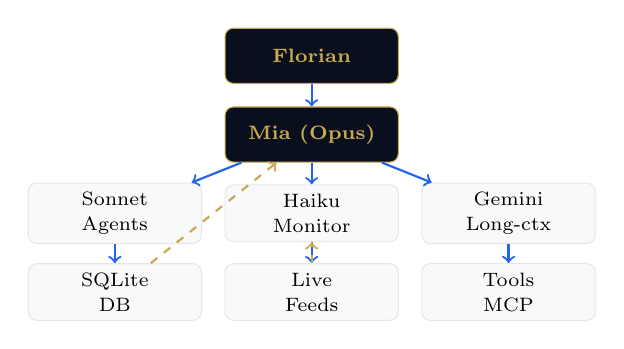
\begin{tikzpicture}[
  box/.style={draw=border, fill=lightgray, rounded corners=3pt, minimum width=2.2cm, minimum height=0.7cm, font=\fontsize{7}{9}\selectfont, align=center},
  goldbox/.style={draw=gold, fill=darkbg, text=gold, rounded corners=3pt, minimum width=2.2cm, minimum height=0.7cm, font=\fontsize{7}{9}\selectfont\bfseries, align=center},
  arr/.style={->, thick, primary}
]
  \node[goldbox] (florian) at (0,3) {Florian};
  \node[goldbox] (mia) at (0,2) {Mia (Opus)};
  \node[box] (sonnet) at (-2.5,1) {Sonnet\\Agents};
  \node[box] (haiku) at (0,1) {Haiku\\Monitor};
  \node[box] (gemini) at (2.5,1) {Gemini\\Long-ctx};
  \node[box] (db) at (-2.5,0) {SQLite\\DB};
  \node[box] (feeds) at (0,0) {Live\\Feeds};
  \node[box] (tools) at (2.5,0) {Tools\\MCP};
  
  \draw[arr] (florian) -- (mia);
  \draw[arr] (mia) -- (sonnet);
  \draw[arr] (mia) -- (haiku);
  \draw[arr] (mia) -- (gemini);
  \draw[arr] (sonnet) -- (db);
  \draw[arr] (haiku) -- (feeds);
  \draw[arr] (gemini) -- (tools);
  \draw[arr, dashed, gold] (feeds) -- (haiku);
  \draw[arr, dashed, gold] (db) -- (mia);
\end{tikzpicture}

\vspace{2pt}

\section{Implementation Roadmap}

{\fontsize{7.5}{10}\selectfont
\begin{tabularx}{\linewidth}{@{}c l X@{}}
\toprule
\rowcolor{lightgray} \textbf{Week} & \textbf{Action} & \textbf{Impact} \\
\midrule
1 & Model routing rules (Haiku heartbeats) & -40\% Opus usage \\
\rowcolor{lightgray}
1 & Gmail/Calendar integration (gog) & Morning briefings \\
2 & SQLite database (contacts, leads, metrics) & Structured queries \\
\rowcolor{lightgray}
2 & Daily briefing cron (07:30 feeds → Telegram) & Proactive intelligence \\
3 & n8n automation (email → CRM → follow-up) & Zero-drop pipeline \\
\rowcolor{lightgray}
3 & Batch review workflow (2×/day, 15 min) & Unblock send queue \\
4 & Evaluate: 2nd account vs. API for sub-agents & Optimize spend \\
\bottomrule
\end{tabularx}
}

\begin{tipbox}
\textbf{The Compound Effect:} Each layer amplifies the others. Database makes research faster → faster research makes better articles → better articles drive leads → leads go into database → cycle accelerates. \textbf{Target: 2× output/week within 4 weeks.}
\end{tipbox}

\end{multicols}

\vspace{2pt}
{\color{border}\rule{\linewidth}{0.3pt}}
\begin{center}
{\fontsize{7}{9}\selectfont\color{subtitle}Florian Ziesche × Mia · Ainary Ventures · \href{https://ainaryventures.com}{ainaryventures.com}}
\end{center}

\end{document}
